\documentclass[conference]{IEEE_Conference_Template/IEEEtran}
\IEEEoverridecommandlockouts
\usepackage{cite}
\usepackage{amsmath,amssymb,amsfonts}
\usepackage{algorithmic}
\usepackage{graphicx}
\usepackage{float}
\graphicspath{{../plots/}{plots/}{./plots/}}
\usepackage{textcomp}
\usepackage{xcolor}
\usepackage[utf8]{inputenc}

\def\BibTeX{{\rm B\kern-.05em{\sc i\kern-.025em b}\kern-.08em
    T\kern-.1667em\lower.7ex\hbox{E}\kern-.125emX}}

\begin{document}

\title{Trabalho 1\\
\large Balanceador de Carga para um Sistema Distribuído}

\author{\IEEEauthorblockN{Lucas Gomes Bussinger da Silva}
\IEEEauthorblockA{RA: 247314}
\and
\IEEEauthorblockN{Bruno Jambeiro Mesquita}
\IEEEauthorblockA{RA: 260382}
}

\maketitle
\thispagestyle{plain}
\pagestyle{plain}

\section{Resumo}
Este relatório apresenta o projeto, a modelagem analítica e a avaliação por simulação de um balanceador de carga em um sistema distribuído composto por três servidores homogêneos. O sistema foi analisado sob três políticas de despacho: Escolha Aleatória, \textit{Round-Robin} e Fila Mais Curta. O objetivo principal foi comparar o desempenho dessas políticas através do tempo médio de resposta ($E[R]$) e validar as propriedades fundamentais da Teoria das Filas, como a estabilidade do sistema, a conservação de trabalho e a Lei de Little, em diferentes níveis de carga ($\lambda$).

\section{Descrição da arquitetura do balanceador e políticas adotadas}
A arquitetura do sistema simulado é composta por um \textit{dispatcher} (balanceador de carga) responsável por receber todas as requisições que chegam ao sistema e encaminhá-las instantaneamente para um dos três servidores de processamento. O balanceador implementa três políticas de roteamento:
\begin{itemize}
    \item \textbf{Escolha Aleatória}: Cada requisição é encaminhada para um dos três servidores com igual probabilidade ($p_i = 1/3$), de forma totalmente independente das requisições anteriores.
    \item \textbf{\textit{Round-Robin}}: O balanceador distribui as requisições de forma cíclica e determinística, seguindo a ordem 1, 2, 3, 1, 2, 3, garantindo uma distribuição equitativa ao longo do tempo.
    \item \textbf{Fila Mais Curta}: O balanceador consulta o estado de cada servidor no instante da chegada de uma requisição e a envia para aquele com o menor número total de tarefas (esperando na fila somado àquela em execução). Em caso de empate, a escolha entre os empatados é feita aleatoriamente.
\end{itemize}

Do ponto de vista prático e de implementação de software, a arquitetura foi desenvolvida na linguagem Python de forma modular e orientada a objetos. O projeto é dividido em três componentes principais: o arquivo \texttt{classes.py}, que abriga o núcleo do sistema contendo as entidades \texttt{Pacote}, \texttt{Servidor}, \texttt{Balanceador} e a máquina de estados no motor \texttt{Simulador} (baseado em avanços de tempo discreto); o script principal \texttt{simulacoes.py}, que orquestra a execução das réplicas, injeta os diferentes níveis de carga $\lambda$ e processa o rigor estatístico como as métricas de intervalo de confiança; e o módulo \texttt{graficos.py}, dedicado exclusivamente à geração das representações visuais utilizadas neste relatório.

\section{Descrição dos servidores e parametrização do tráfego}
O sistema é constituído por três servidores homogêneos. Cada servidor opera com uma única \textit{thread} de execução e atende as requisições de forma serial sob a disciplina \textit{First Come, First Served} (FCFS). A fila de cada servidor é assumida como ilimitada. A taxa de serviço individual de cada servidor segue uma distribuição exponencial de média $1/\mu = 1.0$ unidade de tempo (u.t.), o que resulta em uma capacidade de atendimento de $\mu = 1.0$ requisição por unidade de tempo para cada nó. 
O tráfego de entrada no sistema segue um processo de Poisson, com tempos entre chegadas independentes e identicamente distribuídos segundo uma distribuição exponencial de parâmetro $\lambda$. Foram realizados experimentos para avaliar o sistema sob diferentes cenários de carga de trabalho, parametrizados pelas taxas de chegada $\lambda \in \{0,6; 1,2; 1,8; 2,4; 2,7\}$, operando em regime estável, e um caso instável em que $\lambda = 3,3$. As simulações foram executadas durante 5000 u.t. por 10 réplicas independentes para garantir confiabilidade estatística (intervalos de confiança de 95\%), com um período de \textit{warm-up} inicial de 500 u.t. que foi devidamente descartado na coleta de métricas estacionárias.

\section{Modelagem Analítica}

\subsection{Independência probabilística entre os servidores (política de escolha aleatória)}

3 Servidores

$N$ = Número de jobs no sistema (3 servidores);

$N_1, N_2, N_3$ = Número de Jobs no servidor 1, 2, 3 respectivamente

$N = N_1 + N_2 + N_3$

Para Independência: a Distribuição Conjunta é igual ao produto das marginais:

$n = n_1 + n_2 + n_3$

$\lambda$ = taxa de requisições de pacotes no sistema

$p_1, p_2, p_3$ = probabilidade de a requisição ser enviada para o servidor 1, 2 e 3.

\begin{align}
&P(N_1 = n_1, N_2 = n_2, N_3 = n_3) \nonumber\\
&= P(N_1 = n_1) \cdot P(N_2 = n_2) \cdot P(N_3 = n_3) \nonumber\\
&\quad (\text{Independência}).
\end{align}

Verificando:
\begin{align}
&P(N_1 = n_1, N_2 = n_2, N_3 = n_3) \nonumber\\
&= P(N_1 = n_1, N_2 = n_2, N_3 = n_3 \mid N = n) \cdot P(N = n) \nonumber\\
&= P(N_1 = n_1 \mid N = n) \cdot P(N_2 = n_2 \mid N = n) \nonumber\\
&\quad \cdot P(N_3 = n_3 \mid N = n) \cdot P(N = n) \nonumber\\
&= \frac{n!}{n_1! \, n_2! \, n_3!} \cdot (p_1)^{n_1} \cdot (p_2)^{n_2} \cdot (p_3)^{n_3} \cdot \frac{e^{-\lambda} \lambda^n}{n!} \nonumber\\
&= \frac{e^{-\frac{\lambda}{3}} \left(\frac{\lambda}{3}\right)^{n_1}}{n_1!} \cdot \frac{e^{-\frac{\lambda}{3}} \left(\frac{\lambda}{3}\right)^{n_2}}{n_2!} \cdot \frac{e^{-\frac{\lambda}{3}} \left(\frac{\lambda}{3}\right)^{n_3}}{n_3!}
\end{align}

Que é justamente a multiplicação das marginais modeladas por processo de Poisson com $\lambda_i = \frac{\lambda}{3}$:
\begin{align}
&P(N_1 = n_1) \cdot P(N_2 = n_2) \cdot P(N_3 = n_3) \nonumber\\
&= \frac{e^{-\frac{\lambda}{3}} \left(\frac{\lambda}{3}\right)^{n_1}}{n_1!} \cdot \frac{e^{-\frac{\lambda}{3}} \left(\frac{\lambda}{3}\right)^{n_2}}{n_2!} \cdot \frac{e^{-\frac{\lambda}{3}} \left(\frac{\lambda}{3}\right)^{n_3}}{n_3!}
\end{align}

Sendo os 3 servidores Independentes entre si sob a Política Aleatória.

\subsection{Servidores em fila $M / M / 1$}

Conforme visto no item (a), pelo teorema da decomposição (splitting) de Poisson, a política aleatória divide o processo de chegadas de taxa $\lambda$ em três processos independentes com taxas $\lambda_i = \frac{\lambda}{3}$. Como os tempos entre chegadas em cada servidor têm distribuição Exponencial (M), o tempo de serviço tem distribuição Exponencial (M) e cada servidor tem 1 thread (1), cada servidor se comporta independentemente como uma fila $M/M/1$ isolada.

\paragraph{Utilização}
$U_i$ = utilização do servidor

$p_0 = (1 - \rho)\rho^0 = 1 - \rho \to$ Probabilidade do servidor estar ocioso

$U_i = 1 - p_0 = \rho = \frac{\lambda_i}{\mu_i} \to$ Probabilidade do servidor estar sendo utilizado (Utilização Média)

\paragraph{Número Médio de requisições no servidor: $E[N_i]$}
\begin{align}
E[N_i] &= \sum_{k=0}^{\infty} k \cdot p_k = \sum_{k=0}^{\infty} k \cdot (1 - \rho) \cdot \rho^k = (1 - \rho) \sum_{k=0}^{\infty} k \rho^k \nonumber\\
&= (1 - \rho)\rho \sum_{k=1}^{\infty} k \rho^{k-1} = (1 - \rho)\rho \frac{d}{d\rho} \left[ \sum_{k=0}^{\infty} \rho^k \right] \nonumber\\
&= (1 - \rho)\rho \left( \frac{1}{1-\rho} \right)^2 = \frac{\rho}{1 - \rho}
\end{align}

\begin{equation}
E[N_i] = \frac{\rho}{1 - \rho} \quad \text{para } \rho < 1
\end{equation}

\paragraph{Tempo médio de resposta: $E[R]$}
pela lei de Little:
\begin{equation}
E[N_i] = \lambda_i \cdot E[R]
\end{equation}

\begin{equation}
E[R] = \frac{E[N_i]}{\lambda_i} = \frac{1}{\mu_i - \lambda_i}
\end{equation}

\paragraph{Tempo médio de requisições na fila: $E[T_Q]$}
\begin{equation}
E[R] = E[T_Q] + \frac{1}{\mu_i}
\end{equation}

\begin{equation}
E[T_Q] = E[R] - \frac{1}{\mu_i}
\end{equation}

\begin{equation}
E[T_Q] = \frac{\rho}{\mu_i - \lambda_i}
\end{equation}

\subsection{Vazão $X$ e utilização $U$ valendo para as três políticas}

\paragraph{Vazão $X$}
Em um sistema estável (onde a taxa de chegada é menor que a capacidade de atendimento, $\lambda < 3\mu$), o sistema é conservador de trabalho, o que significa que nenhuma requisição é descartada. Tudo o que entra no balanceador de carga tem que, eventualmente, ser processado e sair do sistema. Como a taxa de entrada é $\lambda$, a vazão (taxa de saída) será inevitavelmente igual à taxa de chegada: $X = \lambda$. A política de balanceamento (Aleatória, Round-Robin ou Fila Mais Curta) apenas reorganiza a ordem ou o local de espera das requisições, mas não altera o fato de que 100\% das requisições recebidas serão atendidas.

\paragraph{Utilização $U_i$}
A utilização é definida pela fração de tempo que um servidor passa ocupado. O trabalho total que chega ao sistema por unidade de tempo é dado por $\lambda \cdot E[S] = \frac{\lambda}{\mu}$.

Esse trabalho total precisa obrigatoriamente ser absorvido pelo conjunto dos 3 servidores. Como os servidores são homogêneos ($\mu = 1$ para todos) e as três políticas distribuem a carga de forma simétrica e justa a longo prazo (nenhuma delas boicota ou favorece permanentemente um servidor específico), o trabalho total será dividido igualmente entre os três.

Portanto, a utilização média de cada servidor será a divisão do trabalho total por três: $U_i = \frac{\lambda}{3\mu} = \rho$. Isso independe de a requisição ter sido enviada por sorteio, de forma cíclica ou para a menor fila.

Como apontado na aula, a política de balanceamento afeta a variabilidade e, consequentemente, altera apenas o tempo de resposta $E[R]$ e o tamanho da fila $E[N]$. A vazão e a utilização independem da política.

\section{Resultados e discussão}
Para avaliar a exatidão da simulação, os resultados empíricos da política Aleatória foram inicialmente contrastados com o modelo analítico $M/M/1$. Observou-se que o modelo simulado da política Aleatória apresenta concordância estatística rigorosa com a curva analítica esperada: $E[R] = \frac{1}{\mu - \lambda/3}$, validando o simulador.

Comparando as três políticas implementadas (Figura \ref{fig:comparacao}), os resultados simulados revelam um ganho progressivo de desempenho na medida em que a inteligência de roteamento se torna menos cega ao estado do sistema. Em todos os cenários de carga observados, verificou-se a ordenação de eficiência: $E[R]_{\text{Fila curta}} \leq E[R]_{\text{Round-Robin}} \leq E[R]_{\text{Aleatória}}$.
\begin{figure}[H]
\centerline{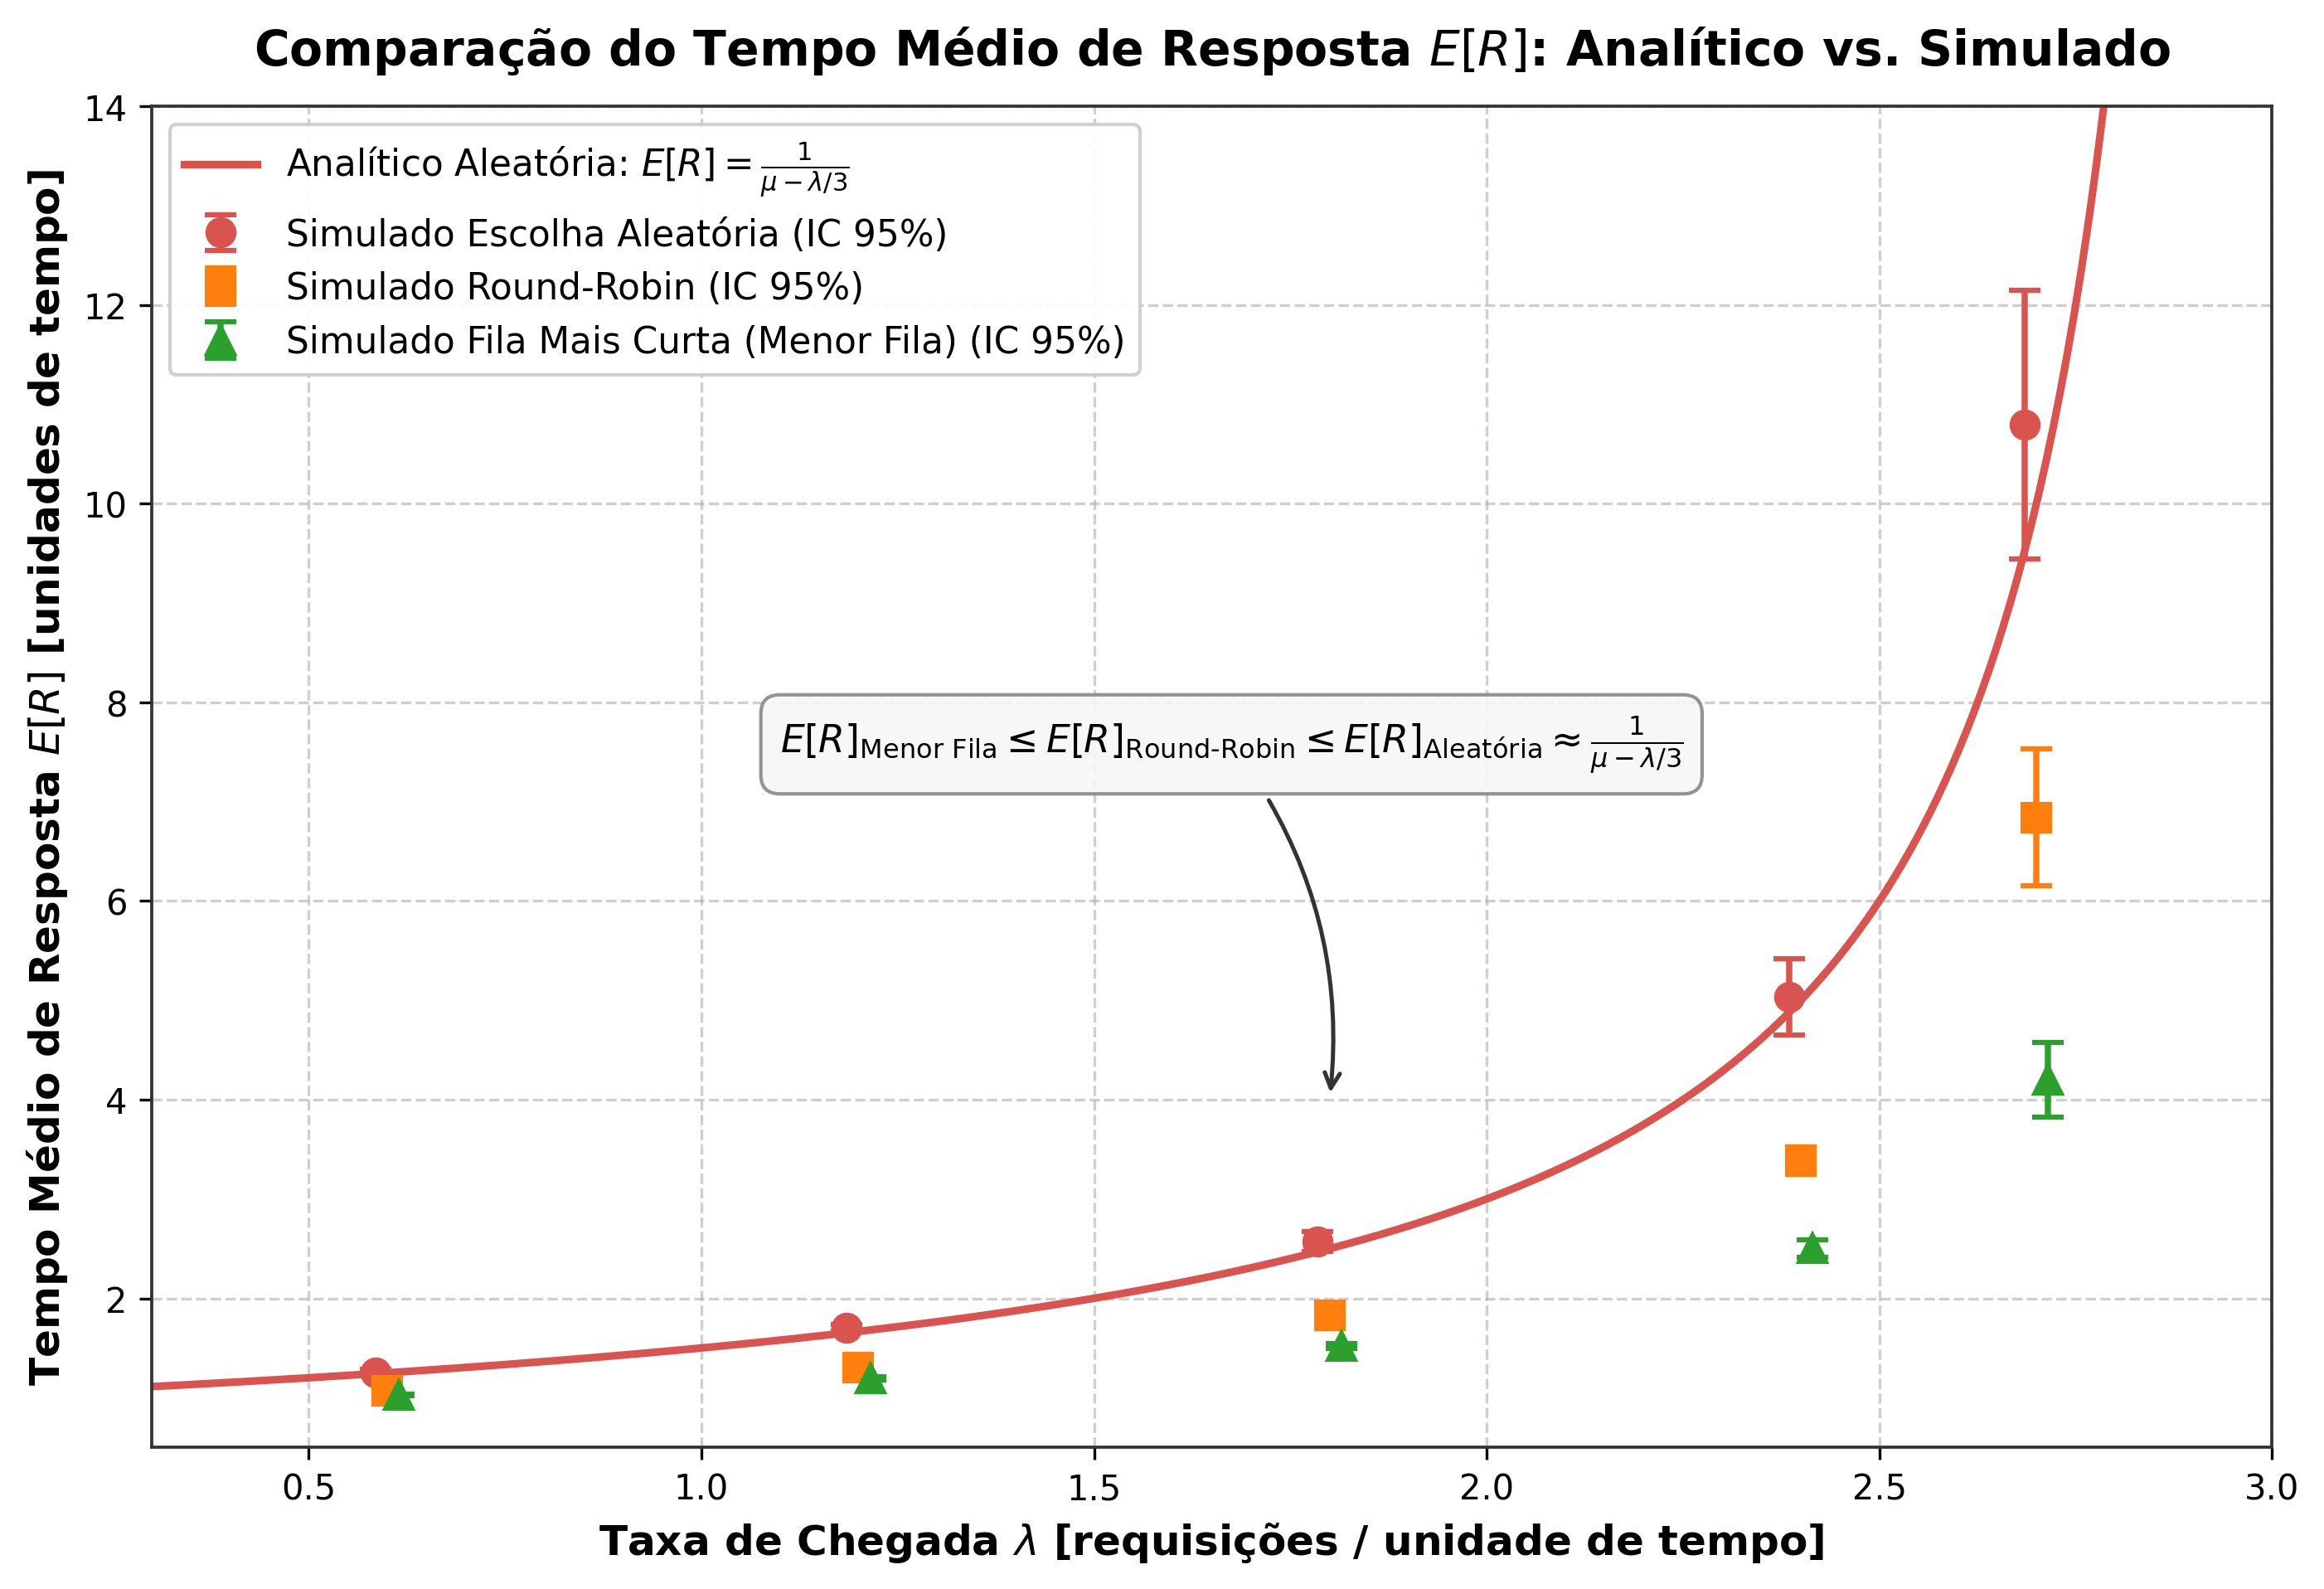
\includegraphics[width=0.8\columnwidth]{../plots/comparacao_politicas_ER.png}}
\caption{Comparação de $E[R]$: Analítico x Simulado.}
\label{fig:comparacao}
\end{figure}

A justificativa para tal fenômeno reside na redução da variância dos tempos entre chegadas percebidos pelos servidores e na minimização de picos localizados de congestionamento. Enquanto a escolha aleatória permite colisões sequenciais no roteamento em curtos espaços de tempo (agravando filas), a política \textit{Round-Robin} determiniza a distribuição das chegadas, atenuando os surtos em cada fila. Contudo, é a política da Menor Fila que atinge o desempenho ótimo neste arranjo por considerar ativamente o inventário instantâneo de pacotes de cada servidor antes de tomar uma decisão, impedindo que requisições repousem em filas de servidores ocupados enquanto houver servidores ociosos. É notório que o ganho percentual dessas políticas sobre a aleatória amplifica-se expressivamente para cargas maiores, onde o congestionamento é mais crítico. Em $\lambda=2,7$, a Menor Fila proporciona um decréscimo de mais de 60\% no tempo de espera em relação ao modelo aleatório puro.

Ademais, demonstrou-se empíricamente a universalidade da Lei de Little ($E[N] = X \cdot E[R]$) para todas as políticas, ilustrada na Figura \ref{fig:little}. Os resultados atestam, com erro inferior a 1\% em todas as configurações, que o tempo que os pacotes aguardam pelo sistema está intrinsecamente ligado à ocupação espacial medida pela área sob a curva das filas.

\begin{figure}[H]
\centerline{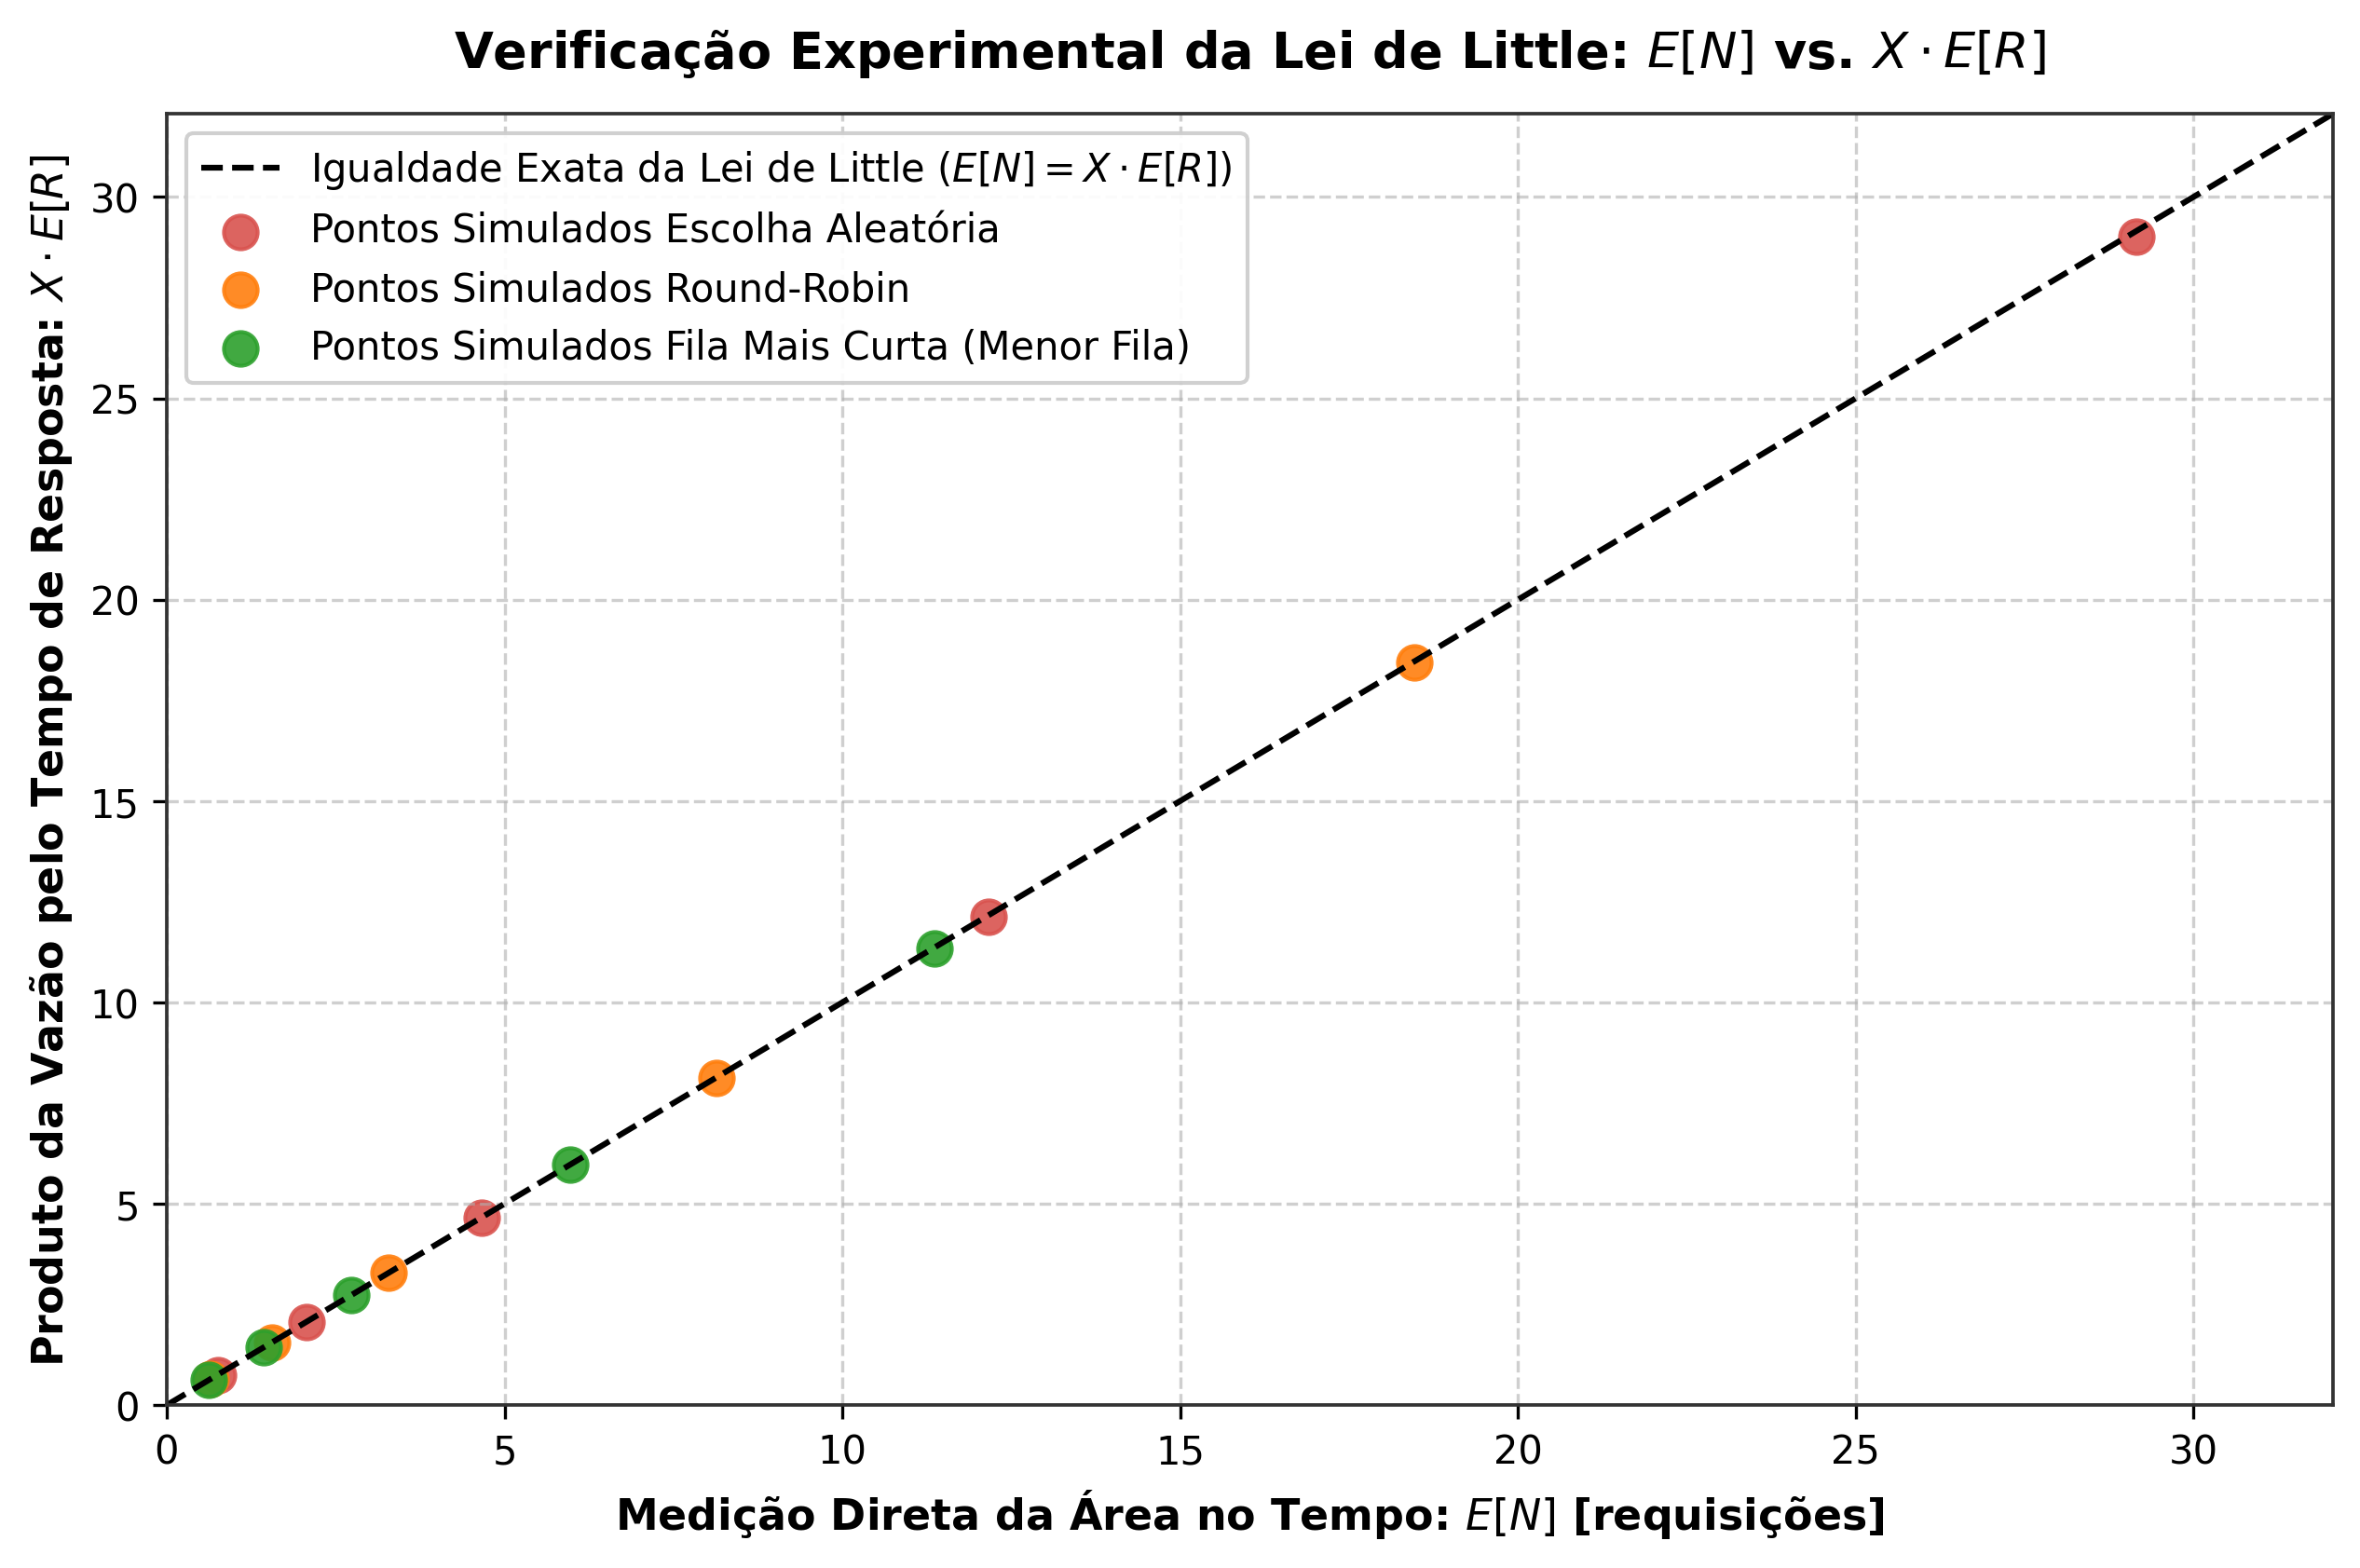
\includegraphics[width=0.8\columnwidth]{../plots/verificacao_lei_de_little.png}}
\caption{Verificação da Lei de Little.}
\label{fig:little}
\end{figure}

Por fim, ao submeter o sistema a uma taxa de chegadas $\lambda=3,3$ maior do que sua capacidade agregada de escoamento $3\mu = 3,0$, as fórmulas analíticas perdem fundamentação uma vez que a condição de estabilidade $\rho = \frac{\lambda}{3\mu} < 1$ não é satisfeita. Nesse regime, a simulação demonstra o colapso gradual do desempenho. Como $\rho > 1$, o sistema passa a acumular $\lambda - 3\mu = 0,3$ requisições permanentemente por unidade de tempo, sendo perfeitamente descrito pela aproximação fluida $N(t) \approx N(0) + (\lambda - 3\mu)t$.





\section{Conclusão}
As simulações computacionais evidenciaram com sucesso o impacto que estratégias de distribuição de carga geram no tempo de resposta percebido pelo cliente em sistemas distribuídos sob alto fluxo. Conclui-se que o compartilhamento dinâmico de estado instantâneo – inerente à estratégia de Menor Fila – mitiga significativamente o fenômeno natural de estrangulamento por filas, apresentando resiliência superior à elevação drástica de demanda quando comparada às estratégias independentes de estado. Adicionalmente, verificaram-se empiricamente premissas sólidas da Teoria de Filas, consolidando o entendimento de que em regimes estacionários de sistemas não-preemptivos de conservação de trabalho, a vazão e a utilização independem da política, evidenciando o tempo de espera como foco central de otimização por meio do \textit{dispatcher}.

\end{document}
